\section{Method}
\subsection{General method for collecting a JSI}
Here the methodology and equipment choices of the performed experiments are described. The logical place to begin is with the silicon chips, which are the central object of interest in the experiments. The chips used were had a typical area of \SI{1}{\centi\meter^2} and a thickness of a few millimetres. In order to couple light into the waveguides etched onto the chip spot size converters or diffraction gratings are used. For spot size converters figure \ref{sideCoupling} shows the procedure. The fibre which directs the light is called a lense fiber, it has a focal point a few micrometers in front of its tip, allowing high accuracy coupling onto the converters. For this type of coupling peizometers were used with a recoupling algorithm which maximised the transmission of light through the chip.
\newline

\begingroup
    \centering  
    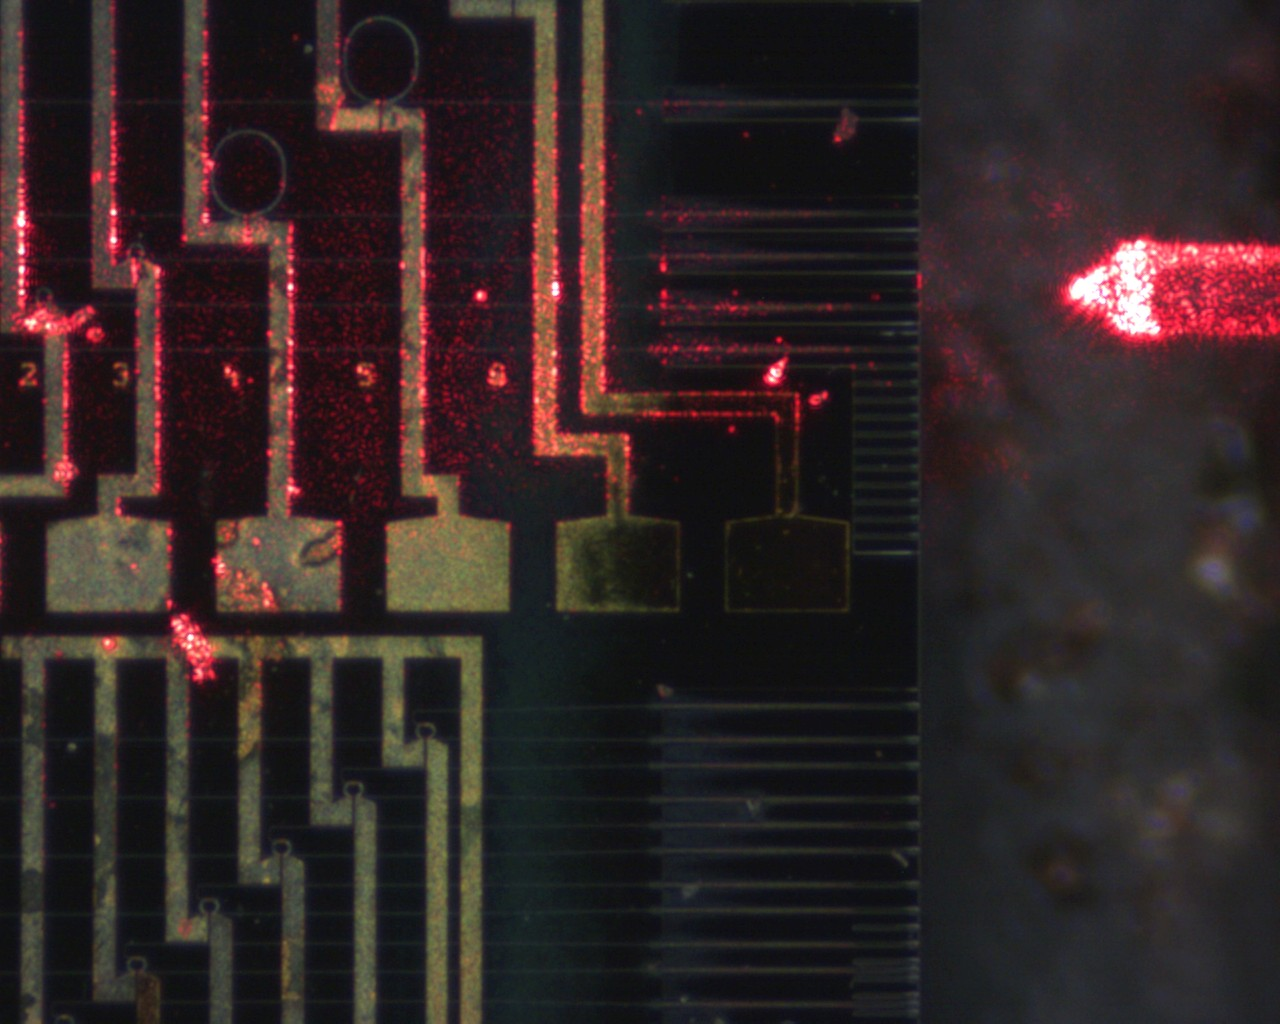
\includegraphics[width=5.3cm]{img/method/chipPictures/redLaser_aboveChip.jpg}
    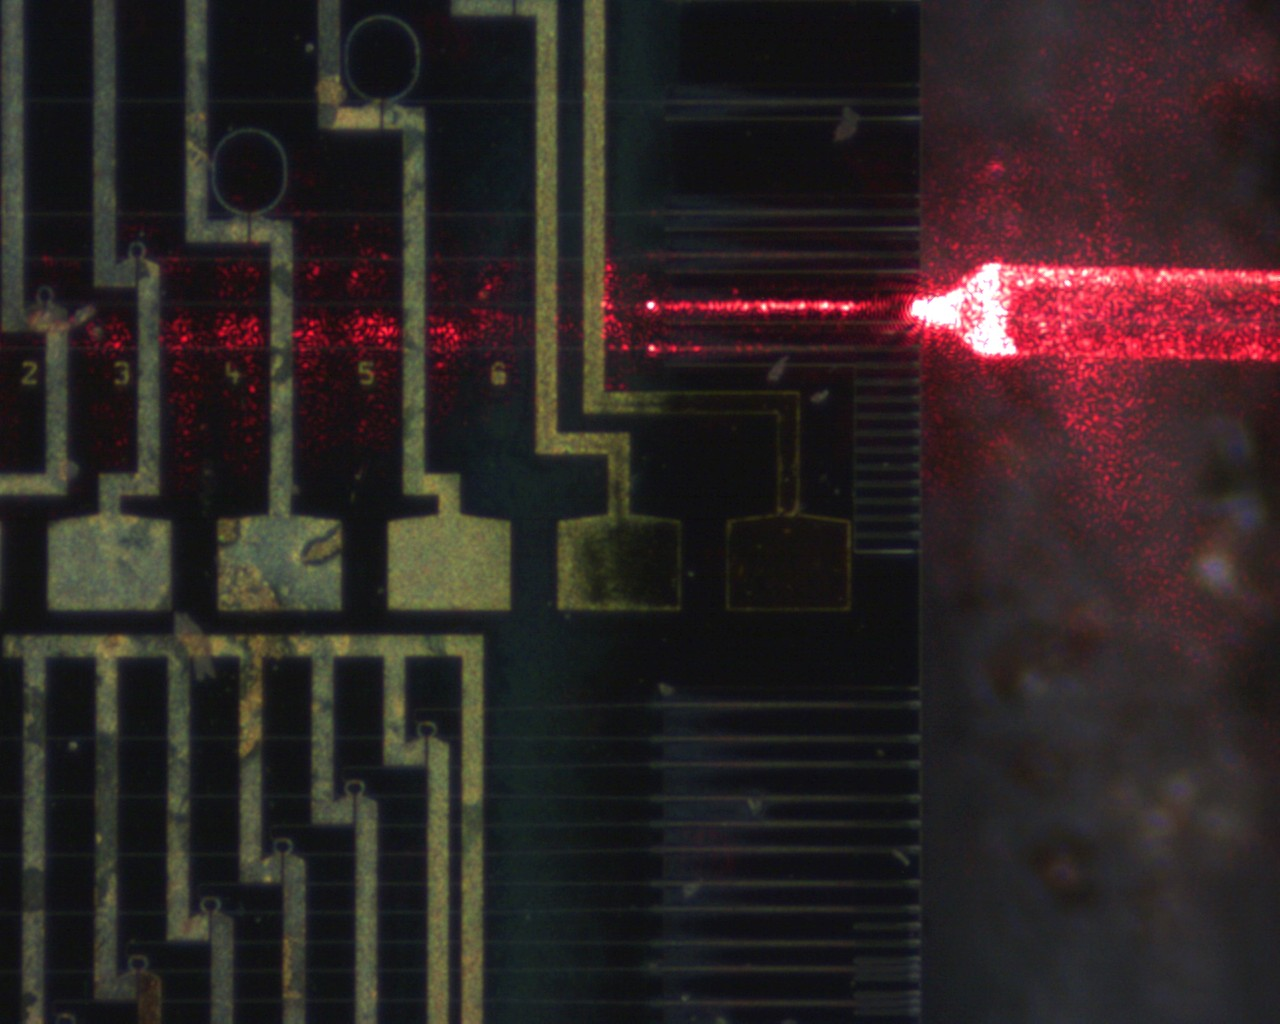
\includegraphics[width=5.3cm]{img/method/chipPictures/redLaser_coupled.jpg}
    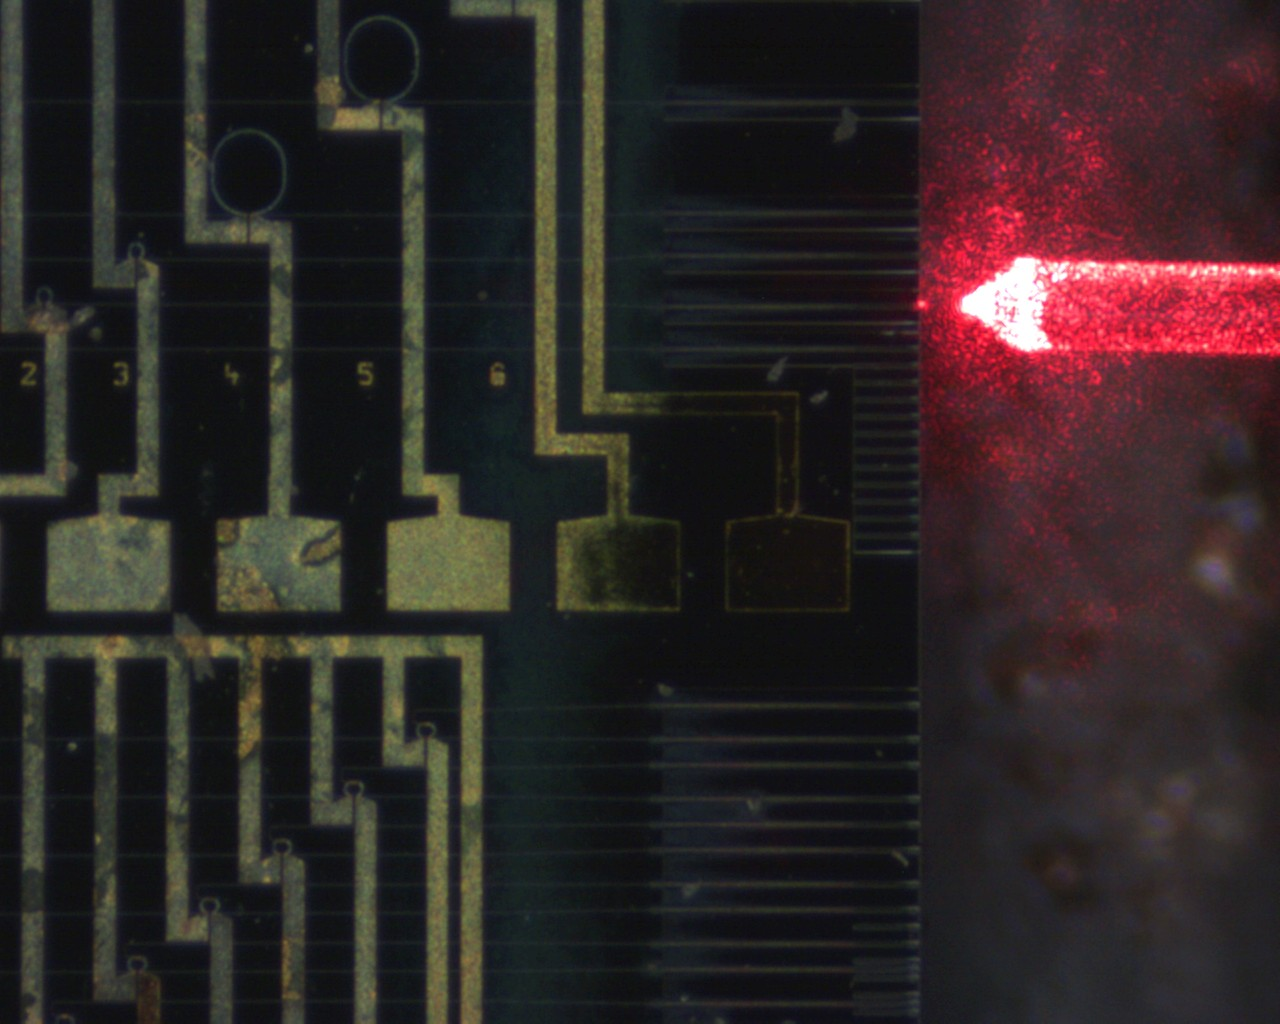
\includegraphics[width=5.3cm]{img/method/chipPictures/redLaser_belowChip.jpg}
    \captionof{figure}{The first image shows the lense fiber above the chip, illuminating its surface, then the fiber has found a good coupling position and finally it is too far underneath the chip. Red light is used for convenience and all other work is done with infared light.}
     \vspace{3pt} \label{sideCoupling}
\endgroup

The second way of getting light into a chip is via diffraction gratings, these are small structures which couple light into a waveguide, figure \ref{verticalCoupling} shows this process from two views. Here the ideal coupling region is much larger, so there is no need for computer control and manual adjustment can suffice.
\newline

\begingroup
    \centering  
    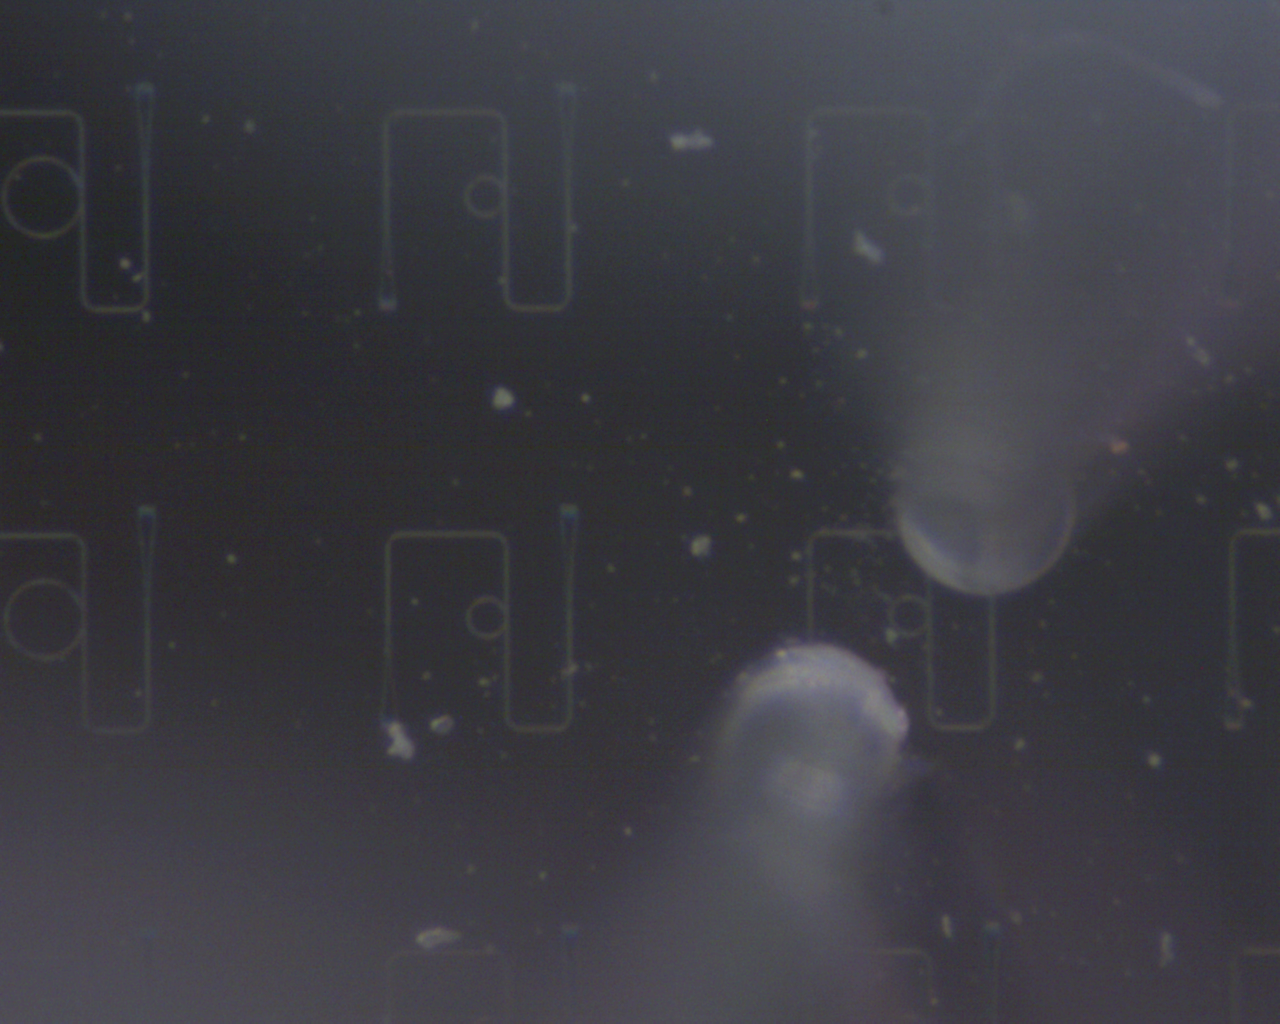
\includegraphics[width=7cm]{img/method/chipPictures/verticalCouplingTopView.png}
    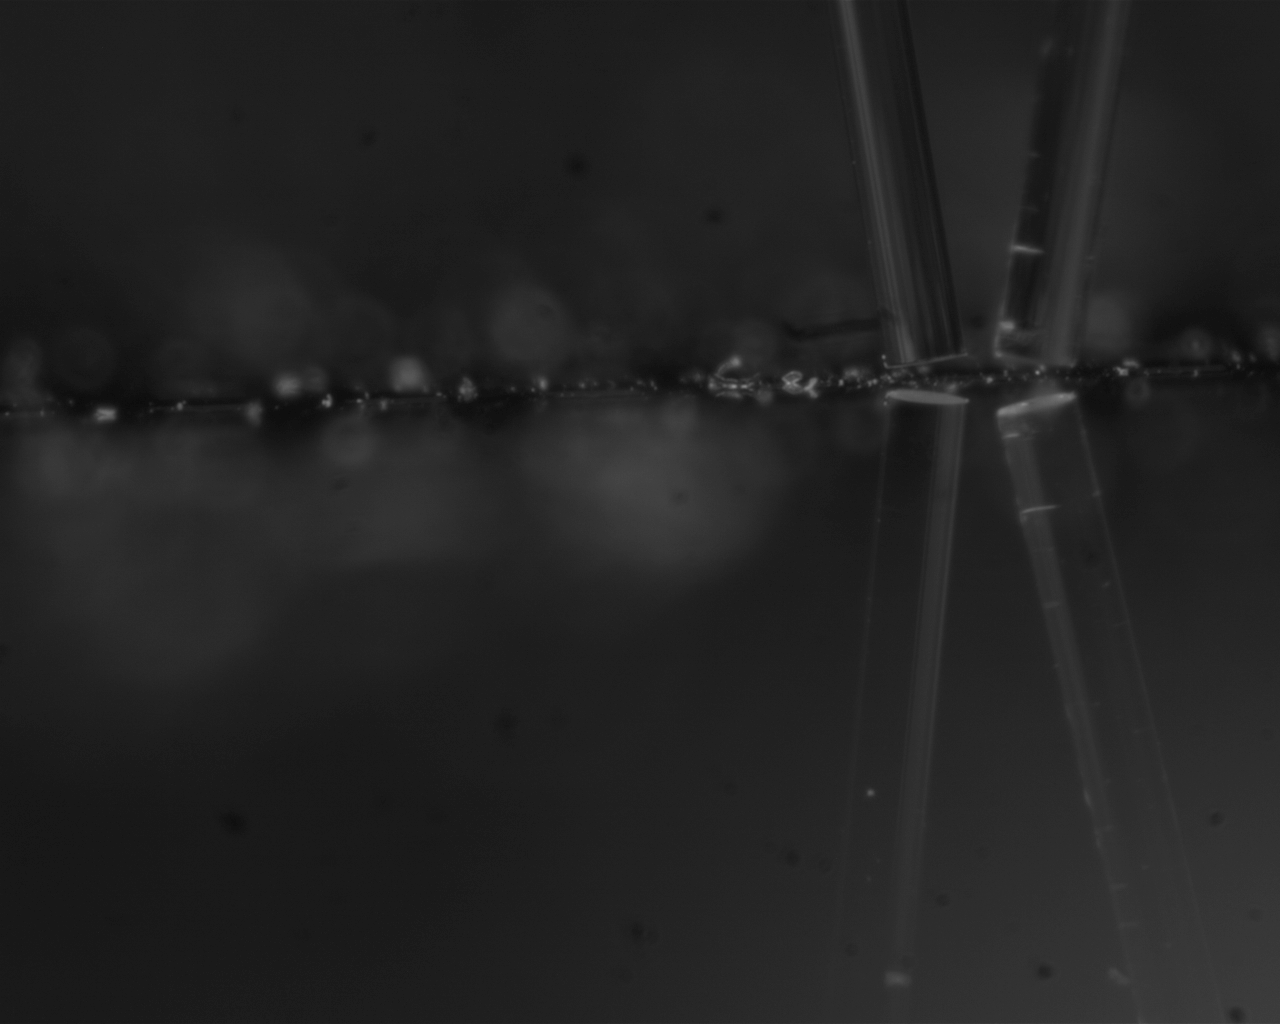
\includegraphics[width=7cm]{img/method/chipPictures/verticalCouplingSideView.png}
    \captionof{figure}{Side coupling proceedure}
     \vspace{3pt} \label{verticalCoupling}
\endgroup

All of these coupling techniques rely on powermeters in the infrared region to maximise the transmission through the chip. Further the polarisation of the light must be adjusted to be inline with the mode which the devices is designed for. 

With light reliably coupled into the chip a spectral scan of the wavelength range \SI{1530}{\nano\meter}-\SI{1560}{\nano\meter} is typically performed to get a transmission spectra like in figure \ref{ringResTrans}. With this the quality factor and the coupling coefficients of the particular ring can be calculated. 

To begin the process for collecting a joint spectrum, the set up is arranged as in figure \ref{simpleJSI}. This maintains the ability to do the above initial procedure. The two powermeters allow the loss due to coupling to be monitored. This is typically on the order of \SI{20}{\deci\bel\m}. 

\begingroup
    \centering  
    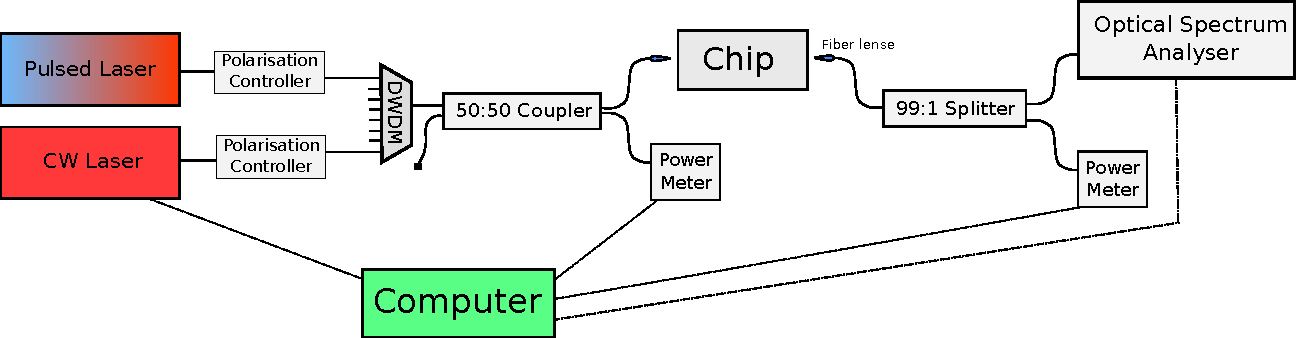
\includegraphics[width=18cm]{img/method/setup_1.pdf}
    \captionof{figure}{Glassgow test structure chip}
     \vspace{3pt} \label{simpleJSI}
\endgroup

The wavelength division multiplexer (DWDM) has 16 channels with \SI{90}{\deci\bel\m} noise suppression and FWHM of \SI{1}{\nano\m}. These are used to suppress the frequency independant background noise caused by amplified spontaneous emission (ASE) in both lasers produce. With temperature control of the chip the resonances are tuned to the center of the DWDM channels. Then two resonances are chosen, onto one the pump is tuned and the other is connected to the CW laser in preparation for the stimulated four wave mixing. 

Figure \ref{aSiBigPicture} is a key illustration of this experiment. With the pulsed laser tuned to a resonance in wavelength and polarisation the CW laser can stimulate the four wave mixing process. 

\begingroup
    \centering  
    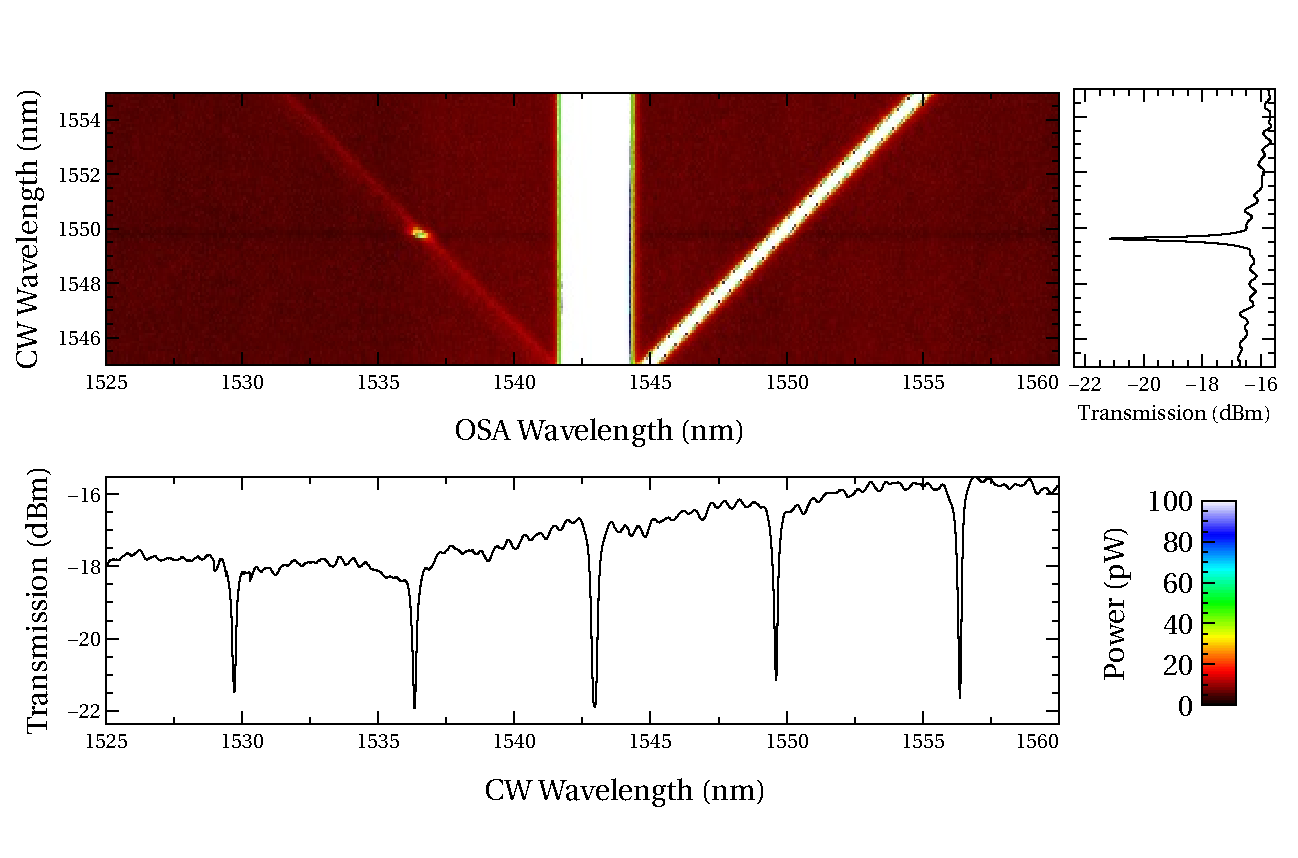
\includegraphics[width=18cm]{img/method/aSiBigPicture.pdf}
    \captionof{figure}{A illustrative example which showing the whole experiment. }
     \vspace{3pt} \label{aSiBigPicture}
\endgroup

Each horizontal slice of figure \ref{aSiBigPicture}   is a sweep on the optical spectrum analyser (OSA). An important experimental decision here is which settings use on the OSA. key settings to be considered for the MS9740A Optical Spectrum Analyzer used are:
\begin{itemize}
	\item \textbf{Video Bandwidth} (VBW) - The OSA functions by passing light through a diffraction grating and then collecting light for some time at each angle, the VBW represents how long it takes for the whole range of wavelengths to be scanned. The OSA has VBW ranging between 1MHz and 10Hz. For the low intensity nature of the signal we are measuring, 10Hz (32s sweep time, \SI{-80}{\decibel\m} sensitivity) and 100Hz (32s sweep time, \SI{-90}{\decibel\m} sensitivity) are typically used.
	\item \textbf{Resolution} - The aperture  which scans across the light coming out of the diffraction grating has a variable size, its minimum is 0.03nm and this was always used to try and achieve the most accurate measurements. 
	\item \textbf{Point Average} - This is how many times each point is measured, useful for eliminating noise.
	\item \textbf{Sweep Average} - This is how many times the OSA sweeps across the spectrum, this also reduces noise. 
	\item \textbf{Number of sample points} - Must be slightly above the resolution in order not to have interpolated data.
	\item \textbf{Wavelength} - The range of wavelengths to be scanned.
\end{itemize}

All of these parameters effect the amount of time it takes to collect a slice of the JSI and hence how long the overall experiment takes. Of course the longest possible integration time will give the best result in theory, but due to decoupling caused by drift in the lense fiber positions and variations in temperature throughout the set up there is limit to the duration of the experiments. 

With the computer controlled coupling it would have been possible to implement a continuous recoupling algorithm during the experiment, however due to the already fairly complex code this was not completed. 

We now summarise the experimental procedure: 

\begin{itemize}
	\item Optimize coupling on both input and output lense fibers
	\item Optimize the polarisation of both input lasers
	\item Temperature tune the resonances to align with the filter channels
	\item Take spectral scans and record initial state
	\item Launch the \lstinline$jointSpectrum$ program which increments the CW laser wavelength and collects OSA spectrums in series. This program also collects some spectrums without the CW laser on for removal of noise.
\end{itemize}

\subsection{Collecting JSI's for varying power}



\begingroup
    \centering  
    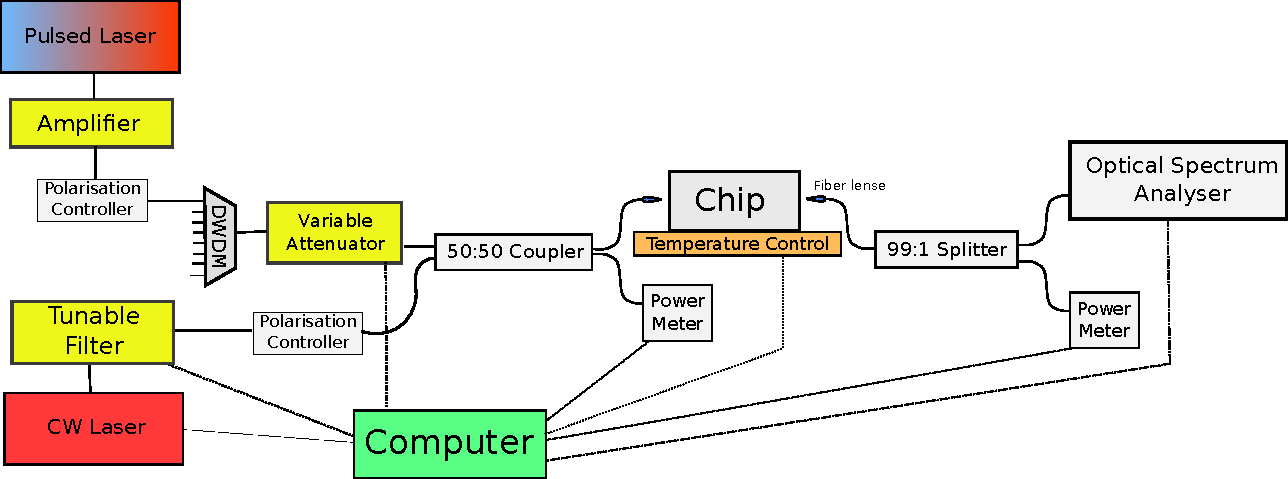
\includegraphics[width=18cm]{img/method/setup_2.pdf}
    \captionof{figure}{big experiment}
     \vspace{3pt} \label{bigJSIExp}
\endgroup




\begingroup
    \centering  
    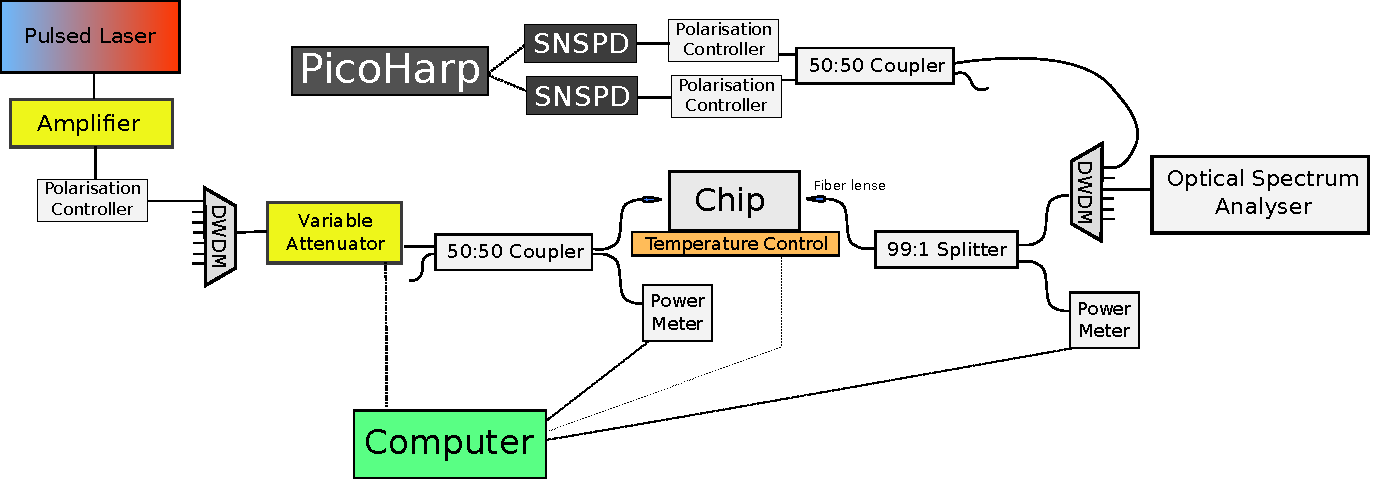
\includegraphics[width=18cm]{img/method/setup_3.pdf}
    \captionof{figure}{single photon}
     \vspace{3pt} \label{crossCompare3}
\endgroup

% Side/Vertical coupling
% Coupling loss
% Blowing up chips -> tempted to add this as a complaint
%	Particularly on glassgow chip
% Temperature tuning



\subsection{Joint Spectrum}
Take the convention that the {\bf signal} photon is the one we measure and the {\bf idler} is the one we stimulate.
% OSA Resolution discussion might be important. Because I think it might have skrewed me over somewhat.
% Filtering
% Could reference the model so that I don't have to use example data.
% Breif description of how this works.
% The algortihm reflects how using narrow filters increases the purity well
% SNR
% NOISE
% NORALISATION
% SPM
% RING DEFORMATION
% How to calculate Q, r, tau
% Comparing with the simulation

% I want to really discuss what we can hope to keep constant and what we can vary. Where you need to really do som engineering to get insights.

\begingroup
    \centering  
    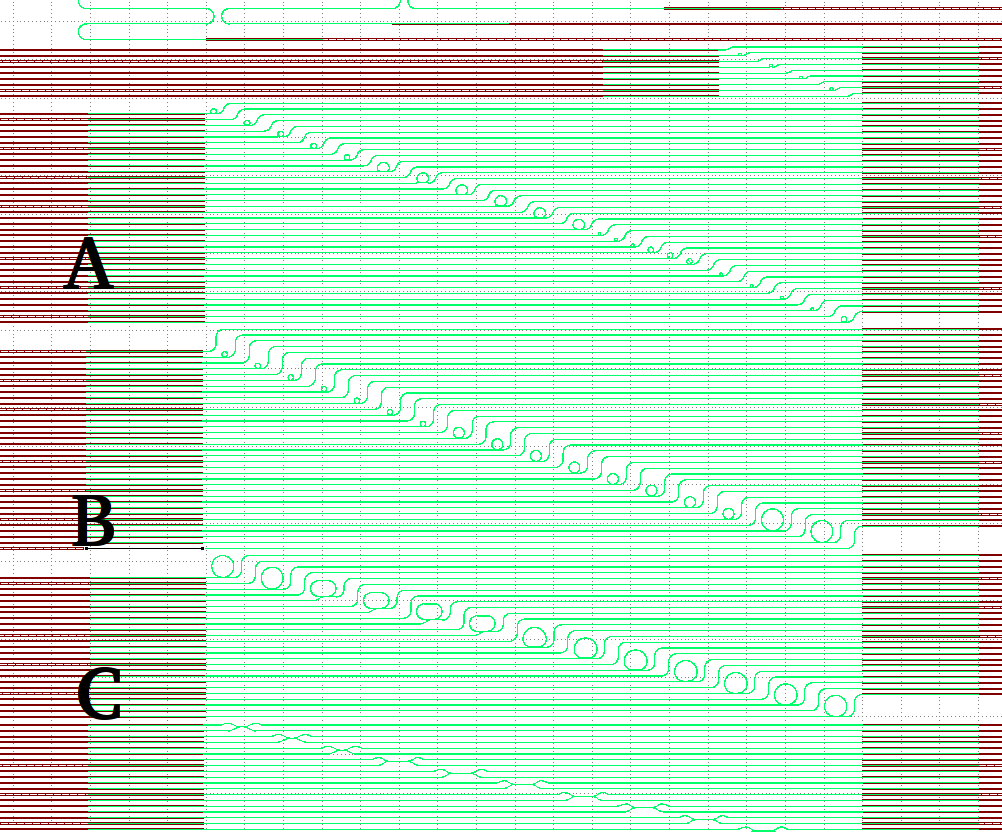
\includegraphics[width=10cm]{img/method/glassgowChipNumbering.png}
    \captionof{figure}{Glassgow test structure chip}
     \vspace{3pt} \label{crossCompare1}
\endgroup

\begingroup
    \centering  
    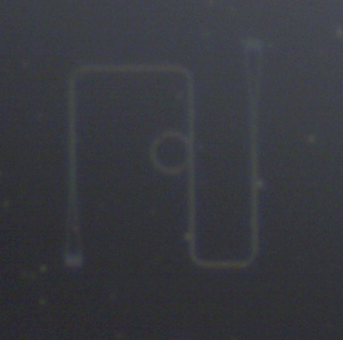
\includegraphics[width=10cm]{img/method/chipPictures/exampleASIRing.png}
    \captionof{figure}{Glassgow test structure chip}
     \vspace{3pt} \label{crossCompare2}
\endgroup